
\documentclass[12pt,aspectratio=169]{beamer}

% Packages
\usepackage{mathtools}
\usepackage{hyperref}
\usepackage{setspace}
\usepackage{tikz}
\usetikzlibrary{positioning}
\usepackage{ragged2e}
\usepackage{nicematrix}
\usepackage[compatibility=false]{caption}
\usepackage[framemethod=tikz]{mdframed}

% Colored boxes
\usepackage{tcolorbox}
\tcbsetforeverylayer{autoparskip} % Removes unwanted vertical space

% Theme
\usetheme{metropolis}
\metroset{subsectionpage=progressbar,sectionpage=none}
\setbeamertemplate{theorems}[numbered]

\usepackage{fontspec}
\defaultfontfeatures{LetterSpace=30}
\usepackage{microtype}

% Prefer flexible inter-word spacing over splitting words across lines.
\tolerance=1
\emergencystretch=\maxdimen
\hyphenpenalty=10000
\hbadness=10000


% Code
\usepackage{listings}
% Custom colors
\definecolor{codegreen}{rgb}{0,0.6,0}
\definecolor{codegray}{rgb}{0.5,0.5,0.5}
\definecolor{codepurple}{rgb}{0.58,0,0.82}
\definecolor{backcolour}{rgb}{0.95,0.95,0.92}
\definecolor{light-gray}{gray}{0.95}
% Python style for highlighting
\newcommand\pythonstyle{\lstset{
		backgroundcolor=\color{white},
		language=Python,
		basicstyle=\ttfamily\footnotesize,
		morekeywords={self},              % Add keywords here
		keywordstyle=\color{blue},
		stringstyle=\footnotesize\color{deepgreen},
		commentstyle=\color{codegreen},
		showstringspaces=false,
		frame=tb,
		numbers=left,
		numbersep=5pt,
		numberstyle=\tiny\color{gray},
		columns=fullflexible,
		numbersep=5pt,
		aboveskip=1em,
		showtabs=false,
		tabsize=2,
		gobble=3
	}}

% Python environment
\lstnewenvironment{python}[1][]
{
	\pythonstyle
	\lstset{#1}
}
{}
% Python for inline
\newcommand\pythoninline[1]{{\pythonstyle\lstinline!#1!}}

% Tables and justification
\newcommand{\ra}[1]{\renewcommand{\arraystretch}{#1}}
\justifying

% Subfigures
\setbeamertemplate{caption}[numbered]
\usepackage[caption=false,font=footnotesize]{subfig}

% Colors
\setbeamercolor{uppercolgreen}{fg=white,bg=green!35}
\setbeamercolor{lowercolgreen}{fg=black,bg=green!10}
\setbeamercolor{uppercolred}{fg=white,bg=red!35}
\setbeamercolor{lowercolred}{fg=black,bg=red!10}
\setbeamercolor{uppercolblue}{fg=white,bg=blue!35}
\setbeamercolor{lowercolblue}{fg=black,bg=blue!10}
\definecolor{darkred}{rgb}{0.55, 0.0, 0.0}
\definecolor{darkpastelblue}{rgb}{0.47, 0.62, 0.8}
\definecolor{darkcerulean}{rgb}{0.03, 0.27, 0.49}
\definecolor{darkgreen}{rgb}{0.0, 0.55, 0.0}
\definecolor{deepblue}{rgb}{0,0,0.5}
\definecolor{deepred}{rgb}{0.6,0,0}
\definecolor{deepgreen}{rgb}{0,0.5,0}

% Matrix size
\usepackage{stackengine}
\stackMath
\def\sss{\scriptstyle \color{gray}}
\setstackgap{L}{12pt}
\def\stacktype{L}

% Mathematical commands
\newcommand{\vc}[1]{\boldsymbol{\mathbf{#1}}}
\newcommand{\pr}[1]{{#1\,}'}
\newcommand{\idx}[2]{{\color{darkpastelblue}[}#1{\color{darkpastelblue}]_{#2}}}
\newcommand{\shape}[2]{\stackunder{#1}{\sss #2}}
\DeclareMathOperator*{\argmax}{arg\,max}
\DeclareMathOperator*{\argmin}{arg\,min}

% Style commands
\newcommand{\myalert}[1]{{\color{darkred}\textbf{#1}}}

% White frame (for images)
\newenvironment{whiteframe}[1]{
	\setbeamercolor{background canvas}{bg=white}
	\begin{frame}{#1}
		}{
	\end{frame}
}

\setbeamerfont{frametitle}{size=\normalsize}
\setbeamertemplate{frametitle}[default][right]
{
}
%\setbeamercolor{frametitle}{fg=white,bg=black!75}

% No headline frame
\makeatletter
\newenvironment{noheadline}{
	\setbeamertemplate{headline}{}
	\addtobeamertemplate{frametitle}{\vspace*{-3.5\baselineskip}}{}
}{}
\makeatother

% Lists
\setbeamertemplate{itemize items}[triangle]

% Footnotes
\setbeamertemplate{footnote}%
{%
	\parindent 1.5em\noindent%
	\justifying\setstretch{0.7}%
	\hbox to 1em{\hfil\insertfootnotemark}\begin{scriptsize}\insertfootnotetext\end{scriptsize}\par%
}

% Footnote without number
\newcommand\blfootnote[1]{%
	\begingroup
	\renewcommand\thefootnote{}\footnote[frame]{\noindent#1}%
	\addtocounter{footnote}{-1}%
	\endgroup
}

% Theorems
\newcommand*{\theorembreak}{\usebeamertemplate{theorem end}\framebreak\usebeamertemplate{theorem begin}}
\newcounter{theo}[section]\setcounter{theo}{0}
\renewcommand{\thetheo}{\arabic{section}.\arabic{theo}}

\newenvironment{theo}[2][]{%
	\refstepcounter{theo}%
	\ifstrempty{#1}%
	{\mdfsetup{%
			frametitle={%
					\tikz[baseline=(current bounding box.east),outer sep=0pt]
					\node[anchor=east,rectangle,fill=red!10]
					{\strut Theorem~\thetheo};}}
	}%
	{\mdfsetup{%
			frametitle={%
					\tikz[baseline=(current bounding box.east),outer sep=0pt]
					\node[anchor=east,rectangle,fill=red!10]
					{\strut Theorem~\thetheo:~#1};}}%
	}%
	\mdfsetup{innertopmargin=5pt,linecolor=red!10,%
		linewidth=2pt,topline=true,%
		frametitleaboveskip=\dimexpr-\ht\strutbox\relax
	}
	\begin{mdframed}[]\relax%
		\label{#2}}{\end{mdframed}}

% Shared content names each box group; the course controls its height.
\tcbset{courseheight/.style 2 args={height=#2}}

% The 2024 source used annotate-equations for two optional visual labels.
% Keep the equations portable in the 2026 repository when that package is absent.
\newcommand{\eqnmarkbox}[3][]{#3}
\newcommand{\annotate}[4][]{}

% Colors
\definecolor{titlecolor}{RGB}{245, 242, 238} 
\definecolor{drawgray}{HTML}{666666}
\definecolor{drawgray_l}{HTML}{F5F5F5}
\definecolor{drawblue}{HTML}{6C8EBF}
\definecolor{drawblue_l}{HTML}{DAE8FC}
\definecolor{drawgreen}{HTML}{82B366}
\definecolor{drawgreen_l}{HTML}{D5E8D4}
\definecolor{draworange}{HTML}{D79B00}
\definecolor{draworange_l}{HTML}{FFE6CC}
\definecolor{drawyellow}{HTML}{D6B656}
\definecolor{drawyellow_l}{HTML}{FFF2CC}
\definecolor{drawred}{HTML}{B85450}
\definecolor{drawred_l}{HTML}{EA6B66}
\definecolor{drawviolet}{HTML}{9673A6}
\definecolor{drawviolet_l}{HTML}{E1D5E7}

\graphicspath{{assets/}{../../shared/assets/}}
\begin{document}

{\usebackgroundtemplate{\tikz\node[opacity=0.4,inner sep=0]{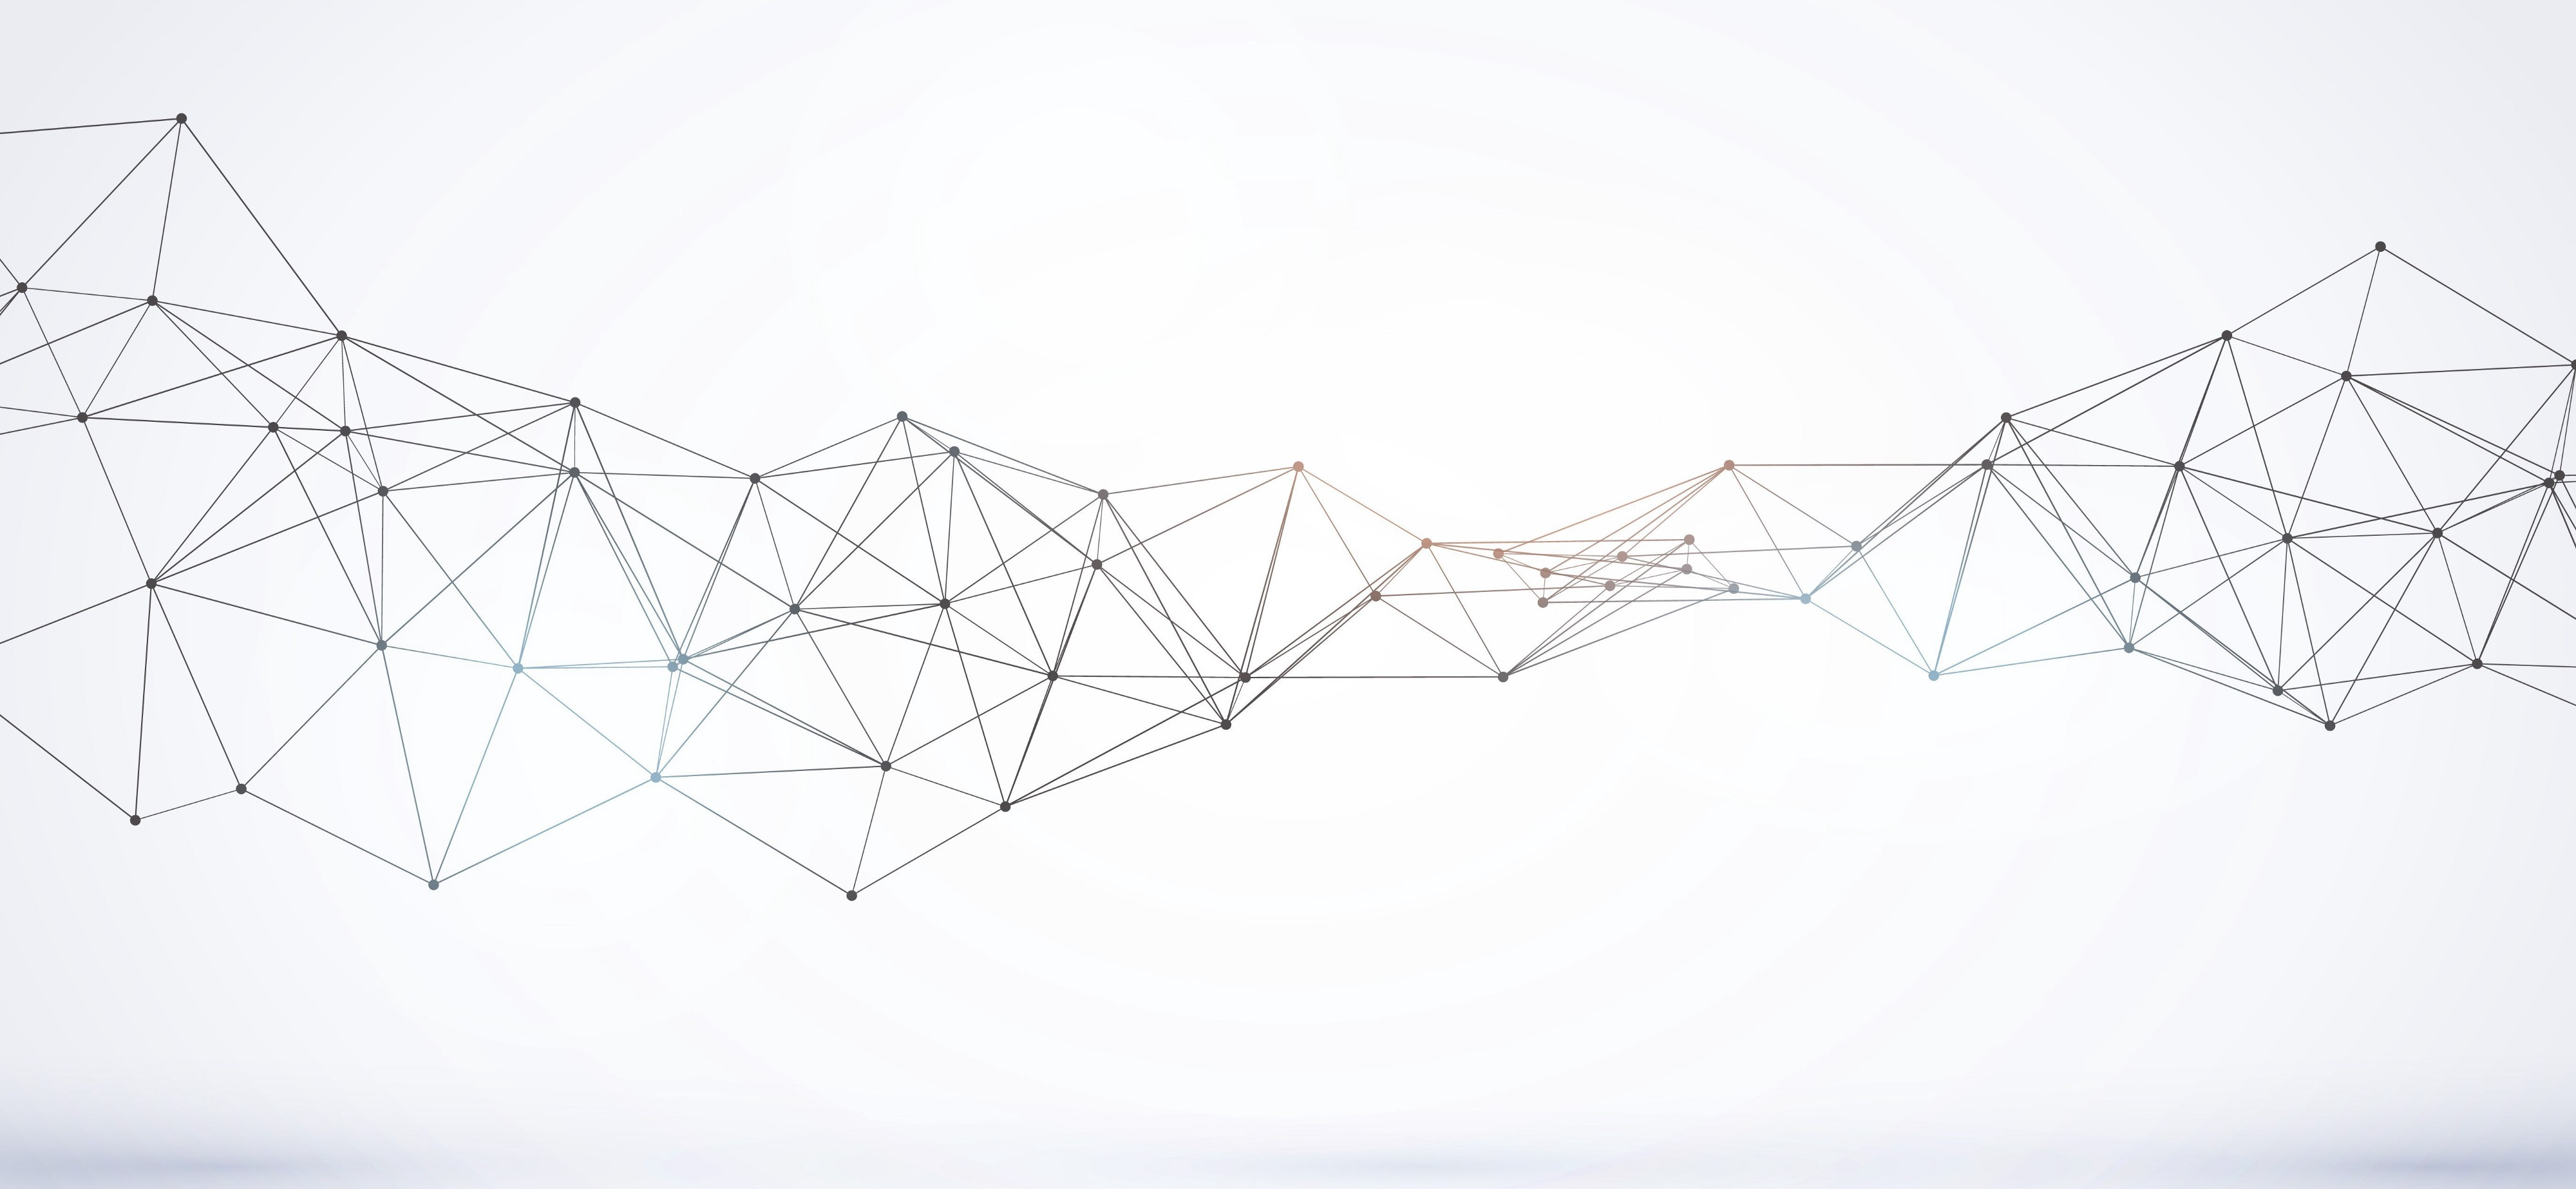
\includegraphics[width=\paperwidth,height=\paperheight]{images/header}};}%
\begin{frame}[plain]
	\vspace{0.5cm}
	\title{\large \begin{spacing}{1.0}Neural Networks for Data Science\end{spacing}\vspace{0.25em}
		\normalsize \begin{spacing}{1.0}\textbf{Master's Degree in Data Science}\end{spacing}\vspace{0.5em}}
	\subtitle{\Large \textbf{Lecture 2: Mathematical preliminaries}\\
		\large 2b. Derivatives and optimization}
	\date{
		{
\includegraphics[scale=0.8]{images/Uniroma1}}
	}
	\author{
		\setlength{\tabcolsep}{2pt}
		\begin{tabular}{rl}
			\textbf{Lecturer}: & S. Scardapane \\
		\end{tabular}
	}\titlepage
\end{frame}
}

\section{Derivatives and gradients}
\subsection{Derivatives and gradients}

\begin{frame}{Empirical risk minimization}

	For a dataset $\left\{x_i, y_i\right\}_{i=1}^N$ (more on this next lecture), let $\boldsymbol{\theta}$ denote the trainable parameters of a model $f_{\boldsymbol{\theta}}(x)$ (e.g., for a linear layer $\boldsymbol{\theta}=\{\vc{W},\vc{b}\}$) and define:
	%
	\begin{equation}
		\mathcal{L}(\boldsymbol{\theta}) =
		\frac{1}{N}\sum_{i=1}^{N}
		\ell\Bigl(f_{\boldsymbol{\theta}}(x_i),y_i\Bigr)\,.
	\end{equation}
	%
	where $\ell$ is some per-example loss. Training is the optimization problem:
	%
	\begin{equation*}
		\boldsymbol{\theta}^* = \argmin_{\boldsymbol{\theta}}\mathcal{L}(\boldsymbol{\theta})\,.
	\end{equation*}

\end{frame}

\begin{frame}{Derivative}

	Most of this course is based on the notion of derivative.

	\begin{tcolorbox}
		The \myalert{derivative} of a function $f(x)$ is defined as:
		%
		\begin{equation}
			\partial f(x) = \frac{\partial}{\partial x}f(x) = \pr{f}(x) = \lim_{h \rightarrow 0} \frac{f(x+h) - f(x)}{h} \,.
		\end{equation}
		%
		Even for a continuous function, $\partial f(x)$ might not be defined everywhere.
	\end{tcolorbox}

	Informally, the derivative expresses the rate of change of $f$ around an infinitesimal displacement from $x$, or the slope of the line tangent to $f(x)$.

\end{frame}

\begin{whiteframe}{Visualizing derivatives in the 1D case}

	\begin{figure}
		\centering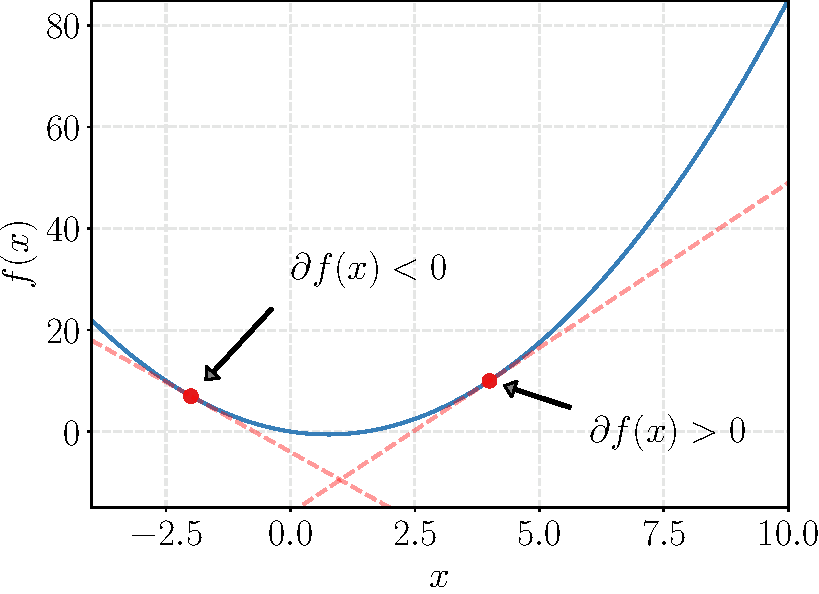
\includegraphics[width=8cm,keepaspectratio]{images/lecture_2/gradient_info.pdf} %
		\caption{1D function ($f(x) = x^2 - 1.5x$), showing the derivative at two different locations.}
	\end{figure}

\end{whiteframe}

\begin{frame}{Properties of derivatives}

	Derivatives possess a number of properties, most notably:
	%
	\begin{itemize}
		\item \textbf{Linearity}: $$ \partial \Big[{\color{darkred}f(x)} + {\color{darkgreen}g(x)}\Big] = {\color{darkred}\pr{f}(x)} + {\color{darkgreen}g'(x)} \,. $$
		\item \textbf{Product rule}: $$ \partial\Big[ {\color{darkred}f(x)}{\color{darkgreen}g(x)}\Big] = {\color{darkred}\pr{f}(x)}{\color{darkgreen}g(x)} + {\color{darkred}f(x)}{\color{darkgreen}g'(x)} \,, $$
		\item \textbf{Chain rule} $$ \partial \Big[{\color{darkred}f(}{\color{darkgreen}g(x)}{\color{darkred})}\Big] = {\color{darkred}\pr{f}(}{\color{darkgreen}g(x)}{\color{darkred})}{\color{darkgreen}g'(x)} \,. $$
	\end{itemize}

\end{frame}

\begin{frame}{Gradient}

	For a function $y=f(\vc{x})$, $\vc{x} \in \mathbb{R}^m$, the \myalert{gradient} $\partial f(\vc{x})$ is an $m$-dimensional vector defined as:%
	\begin{equation}
		\idx{\partial f(\vc{x})}{i} = \frac{\partial f(\vc{x})}{\partial x_i} = \lim_{h \rightarrow 0} \frac{f(\vc{x} + h\vc{e}_i) - f(\vc{x})}{h} \,,
	\end{equation}
	%
	where $\vc{e}_i$ is the $i$th standard basis vector:
	%
	\begin{equation*}
		\idx{\vc{e}_i}{j} = \begin{cases} 1 & \text{ if } i=j \\ 0 & \text{otherwise} \end{cases}
	\end{equation*}
	%
	Sometimes we use the alternative notation $\nabla f(\vc{x})$.

\end{frame}

\begin{frame}{Directional derivative}

	\begin{tcolorbox}
		More generally, the \myalert{directional derivative} of $f(\vc{x})$  in the direction $\vc{v}$ is:
		%
		\begin{equation}
			\mathrm{D}_{\vc{v}}f(\vc{x}) = \lim_{h \rightarrow 0} \frac{f(\vc{x} + h\vc{v}) - f(\vc{x})}{h} \,,
		\end{equation}
	\end{tcolorbox}
	%
	It is easy to prove that:
	%
	\begin{equation}
		\mathrm{D}_{\vc{v}}f(\vc{x}) = \langle \nabla f(\vc{x}), \vc{v} \rangle \,.
	\end{equation}
	%
	A partial derivative is a directional derivative in the direction of a standard basis vector.

\end{frame}

\begin{frame}{Gradients and Jacobians}

	Everything extends to vector-valued functions $\vc{y} = f(\vc{x})$, $\vc{x} \in \mathbb{R}^m$, $\vc{y} \in \mathbb{R}^n$:
	%
	\begin{tcolorbox}
		The \myalert{Jacobian} $\stackunder{\partial f(\vc{x})}{\sss (n, m)}$ of $f$ is a matrix defined as:
		%
		\begin{equation}
			\partial f(\vc{x}) = \begin{pmatrix}
				\frac{\partial y_1}{\partial x_1} & \dots  & \frac{\partial y_1}{\partial x_m} \\
				\vdots                            & \ddots & \vdots                            \\
				\frac{\partial y_n}{\partial x_1} & \dots  & \frac{\partial y_n}{\partial x_m} \\
			\end{pmatrix} \,.
		\end{equation}
	\end{tcolorbox}
	%
	For $n=1$, we recover the gradient, while for $m = n = 1$ we recover the standard derivative.

\end{frame}

\begin{frame}{Examples of matrix derivatives}

	Derivative of the inner product:
	%
	\[
		\frac{\partial}{\partial \vc{x}} \langle \vc{x}, \vc{y} \rangle = \vc{y} \,.
	\]

	Derivative of a linear map:
	%
	\[
		\frac{\partial}{\partial \vc{x}} \vc{A}\vc{x} = \vc{A} \,.
	\]

	Derivative of the squared Euclidean norm:
	%
	\[
		\partial \lVert \vc{x} \rVert^2 = 2\vc{x} \,.
	\]

	\blfootnote{See the matrix cookbook for reference: \\ \url{https://www.math.uwaterloo.ca/~hwolkowi/matrixcookbook.pdf}.}

\end{frame}

\begin{frame}{Properties of gradients}

	Jacobians inherit many properties from the scalar case. Importantly, there exists a chain rule for Jacobians. For $f: \mathbb{R}^m \rightarrow \mathbb{R}^n$ and $g: \mathbb{R}^o \rightarrow \mathbb{R}^m$:
	%
	\vspace{0.35cm}

	\begin{center}
	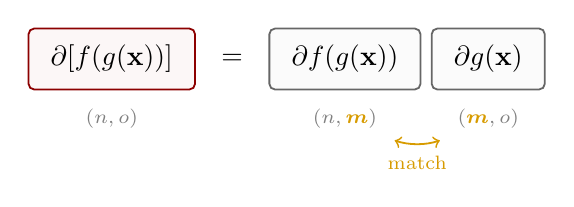
\begin{tikzpicture}[
		node distance=0.22cm,
		every node/.style={font=\normalsize},
		term/.style={
			draw=drawgray,
			line width=0.65pt,
			rounded corners=2pt,
			fill=black!1.5,
			inner xsep=8pt,
			inner ysep=6pt
		},
		result/.style={
			term,
			draw=darkred,
			fill=darkred!3
		},
		dim/.style={font=\scriptsize, text=gray}
	]
		\node[result] (composition)
			{$\partial\!\left[f(g(\vc{x}))\right]$};
		\node[right=0.20cm of composition] (equals) {$=$};
		\node[term, right=0.20cm of equals] (outer)
			{$\partial f(g(\vc{x}))$};
		\node[term, right=0.12cm of outer] (inner)
			{$\partial g(\vc{x})$};

		\node[dim, below=0.11cm of composition]
			{$(n,o)$};
		\node[dim, below=0.11cm of outer] (outer-dim)
			{$(n,\textcolor{draworange}{\boldsymbol{m}})$};
		\node[dim, below=0.11cm of inner] (inner-dim)
			{$(\textcolor{draworange}{\boldsymbol{m}},o)$};

		\draw[
			<->,
			draworange,
			line width=0.65pt,
			shorten <=3pt,
			shorten >=3pt
		]
			(outer-dim.south east)
			to[bend right=18]
			node[below=1pt, font=\scriptsize, text=draworange] {match}
			(inner-dim.south west);
	\end{tikzpicture}
	\end{center}
	\vspace{-0.45cm}
	%
	In words: the Jacobian of the composition of two functions is the product of their Jacobian matrices.

\end{frame}

\begin{frame}{First-order approximation}


	\begin{tcolorbox}
		Given a scalar-valued function $f$ and a reference point $\vc{x}_0$, the best \textbf{linear approximation} of $f$ around $\vc{x}_0$ is given by (\myalert{Taylor's theorem}):
		%
		$$
			\widetilde{f}(\mathbf{x})= f(\mathbf{x}_0)+\langle \eqnmarkbox[drawred]{node}{\partial f(\mathbf{x}_0)}, \eqnmarkbox[drawgreen]{node2}{\mathbf{x}-\mathbf{x}_0} \rangle
			\annotate[yshift=1em]{above,right}{node}{Slope of the line}
			\annotate[yshift=-1em]{below,left}{node2}{Displacement from $\mathbf{x}_0$}
		$$
	\end{tcolorbox}

	\vspace{1em}

	Better approximations can be constructed from higher-order derivatives, but this is enough for building effective optimization algorithms.

\end{frame}

\begin{whiteframe}{Visualizing the approximation}

	\begin{figure}
		\centering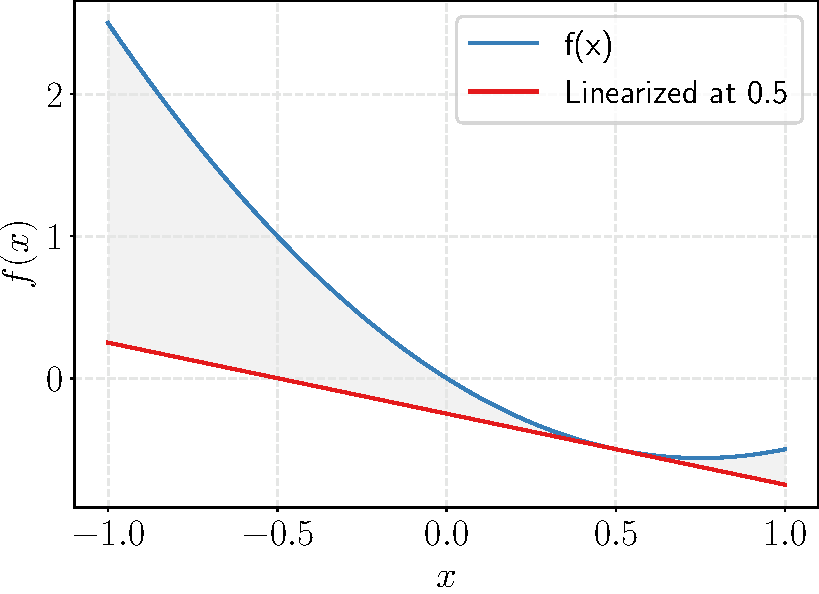
\includegraphics[width=8cm,keepaspectratio]{images/lecture_2/taylor_approximation.pdf} %
		\caption{1D function ($f(x) = x^2 - 1.5x$), linearized at 0.5.}
	\end{figure}

\end{whiteframe}

%\begin{frame}{Taylor's theorem (with remainders)}
%	
%	Taylor's theorem is sometimes shown in an alternative form, which is useful for proofs and for optimization:
%	%
%	\begin{equation}
%		f(\vc{x} + \underbrace{\alpha\vc{h}}_{\mathclap{\text{Small displacement along } \vc{h}}}) = f(\vc{x}) + \alpha \langle \partial f(\vc{x} + \widetilde{\alpha}\vc{h}), \vc{h} \rangle \,,
%	\end{equation}
%	%
%	for some \textit{unknown} $\widetilde{\alpha} \in \left[0, \alpha\right]$. Note that there is no approximation in the result, provided the neighbourhood is sufficiently small.
%	
%	\begin{tcolorbox}
%	\textbf{Important corollary}: if $\langle \partial f(\vc{x}), \vc{h} \rangle < 0$, for suitably small $\alpha$, then $f(\vc{x} + \alpha\vc{h}) < f(\vc{x})$ ($\vc{h}$ is a \myalert{descent direction}).
%	\end{tcolorbox}
%
%\end{frame}

\subsection{Numerical optimization}

\begin{frame}{Optimizing a function}

	We can use gradients to solve generic problems of the form:
	%
	\begin{equation}
		\boldsymbol{\theta}^* = \argmin_{\boldsymbol{\theta}} \mathcal{L}(\boldsymbol{\theta})
	\end{equation}
	%
	Note that maximizing/minimizing are equivalent in the sense that:
	%
	\begin{equation}
		\boldsymbol{\theta}^* = \argmax_{\boldsymbol{\theta}} \mathcal{L}(\boldsymbol{\theta}) = \argmin_{\boldsymbol{\theta}} {\color{darkred} -} \mathcal{L}(\boldsymbol{\theta})
	\end{equation}

\end{frame}

\begin{frame}{A few additional definitions}

	\begin{tcolorbox}
		A point $\boldsymbol{\theta}$ such that $\mathcal{L}(\boldsymbol{\theta}) \le \mathcal{L}(\boldsymbol{\theta}') \;\;\forall\; \boldsymbol{\theta}'$ is called a \myalert{global minimum}. If instead (less restrictive):
		%
		\begin{equation}
			\mathcal{L}(\boldsymbol{\theta}) \le \mathcal{L}(\boldsymbol{\theta}') \;\;\forall\; \boldsymbol{\theta}' \in \left\{ \boldsymbol{\theta}': \lVert \boldsymbol{\theta}' - \boldsymbol{\theta} \rVert^2 < \varepsilon \right\}
		\end{equation}
		%
		for some $\varepsilon > 0$, it is called a \myalert{local minimum}.
	\end{tcolorbox}

	\begin{tcolorbox}
		If $\nabla \mathcal{L}(\boldsymbol{\theta}) = 0$, $\boldsymbol{\theta}$ is called a \myalert{stationary point}. Stationary points can be minima, maxima, or \myalert{saddle points}.
	\end{tcolorbox}

	First-order optimization algorithms return stationary points, which are either local minima or saddle points.

\end{frame}

\begin{whiteframe}{Types of stationary points}

	\begin{figure}
	\centering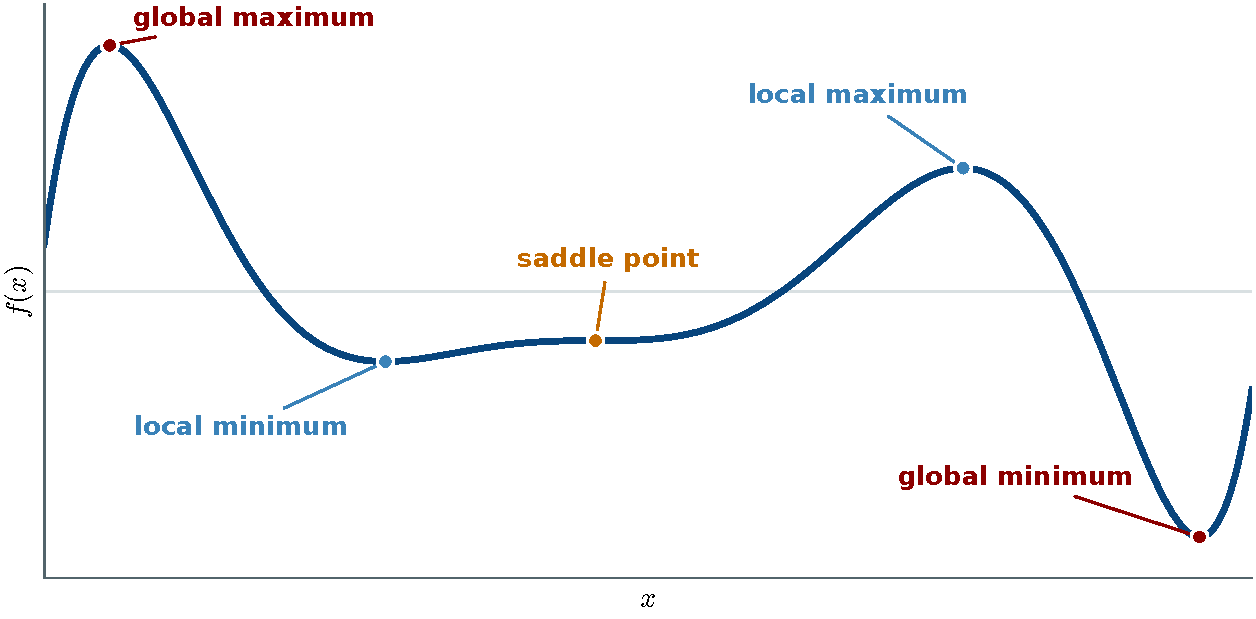
\includegraphics[width=9.5cm,keepaspectratio]{images/lecture_2/stationary_points.pdf} %
	\vspace{-1em}\caption{Stationary points can be \myalert{local} or
		\myalert{global} extrema, or \myalert{saddle points}; here, the saddle
		is a stationary inflection.}
	\end{figure}

\end{whiteframe}

\begin{frame}{Finding stationary points}


	\begin{tcolorbox}

		Given a randomly initialized $\boldsymbol{\theta}_0$, an \myalert{iterative optimization algorithm} has the form:
		%
		\begin{equation}
			\boldsymbol{\theta}_t = \eqnmarkbox[drawred]{node}{\boldsymbol{\theta}_{t-1}} + \eqnmarkbox[drawblue]{node2}{\eta_t\mathbf{p}_t}
			\label{eq:iterative_descent}
			\annotate[yshift=1em]{above,left}{node}{Guess at iteration $t$}
			\annotate[yshift=-1em]{below,left}{node2}{Displacement at iteration $t$}
		\end{equation}
	\end{tcolorbox}

	$\vc{p}_t$ is called a \myalert{descent direction} for $\mathcal{L}(\boldsymbol{\theta}_{t-1})$ if $\mathcal{L}(\boldsymbol{\theta}_t) < \mathcal{L}(\boldsymbol{\theta}_{t-1})$ for a sufficiently small $\eta_t$. $\eta_t$ is called \myalert{step size} or \myalert{learning rate}.

	To implement this iterative algorithm we need a way to choose a descent direction (and a step size) for all $t$.

\end{frame}

\begin{frame}[fragile]{Descent direction}

	We restrict to unit directions, $\lVert\vc{p}_t\rVert=1$.

	\begin{tcolorbox}[
		colback=drawgray_l,
		colframe=drawgray,
		boxrule=0.55pt,
		arc=1.5pt,
		left=5pt,
		right=5pt,
		top=3pt,
		bottom=3pt
	]
		\small
		Recall:
		$\langle\vc{a},\vc{b}\rangle
		=\lVert\vc{a}\rVert\lVert\vc{b}\rVert\cos(\theta)$,
		where $\theta$ is the angle between the vectors.
	\end{tcolorbox}

	\begin{columns}[T,onlytextwidth]
		\begin{column}{0.64\textwidth}
			The rate of change along $\vc{p}_t$ is:
			%
			\small
			\begin{align*}
				\mathrm{D}_{\vc{p}_t}\mathcal{L}(\boldsymbol{\theta}_{t-1})
				&=
				\left\langle
					{\color{darkred}\nabla\mathcal{L}(\boldsymbol{\theta}_{t-1})},
					{\color{darkpastelblue}\vc{p}_t}
				\right\rangle
				\\[0.15em]
				&=
				\left\lVert\nabla\mathcal{L}(\boldsymbol{\theta}_{t-1})\right\rVert
				\underbrace{\lVert\vc{p}_t\rVert}_{=1}
				{\color{draworange}\cos(\theta)}
				\\[0.15em]
				&=
				\left\lVert\nabla\mathcal{L}(\boldsymbol{\theta}_{t-1})\right\rVert
				{\color{draworange}\cos(\theta)}.
			\end{align*}
		\end{column}

		\begin{column}{0.32\textwidth}
			\vspace{0.05cm}
			\centering
			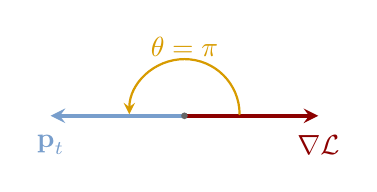
\begin{tikzpicture}[>=stealth, line cap=round]
				\coordinate (origin) at (0,0);
				\draw[
					->,
					darkred,
					line width=1.3pt
				]
					(origin) -- (1.7,0)
					node[below=3pt, text=darkred]
					{$\nabla\mathcal{L}$};
				\draw[
					->,
					darkpastelblue,
					line width=1.3pt
				]
					(origin) -- (-1.7,0)
					node[below=3pt, text=darkpastelblue]
					{$\vc{p}_t$};
				\draw[
					->,
					draworange,
					line width=0.8pt
				]
					(0.70,0.02) arc[start angle=0,end angle=180,radius=0.70];
				\node[text=draworange] at (0,0.88) {$\theta=\pi$};
				\fill[drawgray] (origin) circle (1.2pt);
			\end{tikzpicture}

			\vspace{0.18cm}

			{\small Minimum at ${\color{draworange}\cos(\theta)}=-1$:}

			\vspace{0.12cm}

			$\displaystyle
				\vc{p}_t\propto
				-\nabla\mathcal{L}(\boldsymbol{\theta}_{t-1})$.
		\end{column}
	\end{columns}

	This is the \myalert{steepest descent direction}. More generally,
	anything with $\cos(\theta)<0$ is a descent direction.

\end{frame}

\begin{frame}{Gradient descent}

	The resulting algorithm is called \myalert{gradient descent}.
	%
	\begin{tcolorbox}
		Gradient descent (GD) finds stationary points by iterating:
		%
		\begin{equation}
			\boldsymbol{\theta}_t = \boldsymbol{\theta}_{t-1} - \eta_t \nabla \mathcal{L}(\boldsymbol{\theta}_{t-1}) \,.
		\end{equation}
	\end{tcolorbox}

	This is the basic form of gradient descent (GD, also known as \textbf{first-order} optimization): steepest local directions are not necessarily the \textit{fastest} in general and we can accelerate this iteration in many ways.

\end{frame}

\subsection{Stochastic gradient descent}

\begin{frame}{Handling large datasets}

	Consider the steps needed for a single iteration of GD in our specific optimization problem:

	\begin{enumerate}
		\item Computing the output of the model $f(\vc{x})$ on \textit{all} examples;
		\item Computing the gradient of the cost function with respect to the parameters.
	\end{enumerate}

	Both these operations scale \textit{linearly} in the number of examples, which is unfeasible when we have $10^5$ or even more examples.

	In practice, to train neural networks we use \myalert{stochastic} versions of GD, that approximate the real gradient from smaller amounts of data.

\end{frame}

\begin{frame}{Stochastic GD}

	The key observation is that the training problem in NNs is an average over the full dataset ($\vc{\theta}$ is the set of weights):
	%
	\begin{equation}
		\mathcal{L}(\vc{\theta}) = \frac{1}{N} \sum_{i=1}^N \displaystyle \ell(f_{\boldsymbol{\theta}}(x_i), y_i) \,.
	\end{equation}

	To limit the complexity, we can use only a \myalert{mini-batch} $\mathcal{B}_t$ of $B$ examples randomly sampled from the full dataset:
	%
	\begin{equation}
		\mathcal{L}(\vc{\theta}) \approx \widetilde{\mathcal{L}}_t(\vc{\theta})
		= {\color{darkred}\frac{1}{B} \sum_{i \in \mathcal{B}_t}}
		\displaystyle \ell(f_{\vc{\theta}}(x_i), y_i)\,.
	\end{equation}
	%
	The mini-batch gradient is a (unbiased, noisy) estimate of the full gradient.

\end{frame}

\begin{frame}{Characteristics of stochastic GD}

	The previous algorithm is called \myalert{stochastic gradient descent} (SGD).

	The computational cost of one SGD iteration grows with $B$ (the \myalert{batch size}), but does not depend on the full dataset size $N$ once $B$ is fixed.

	Under standard regularity assumptions and a suitable learning-rate schedule, the noisy mini-batch gradients can still drive the expected gradient norm towards zero.

\end{frame}

\begin{whiteframe}{Full-batch vs. mini-batch trajectories}

	\begin{figure}
		\centering
		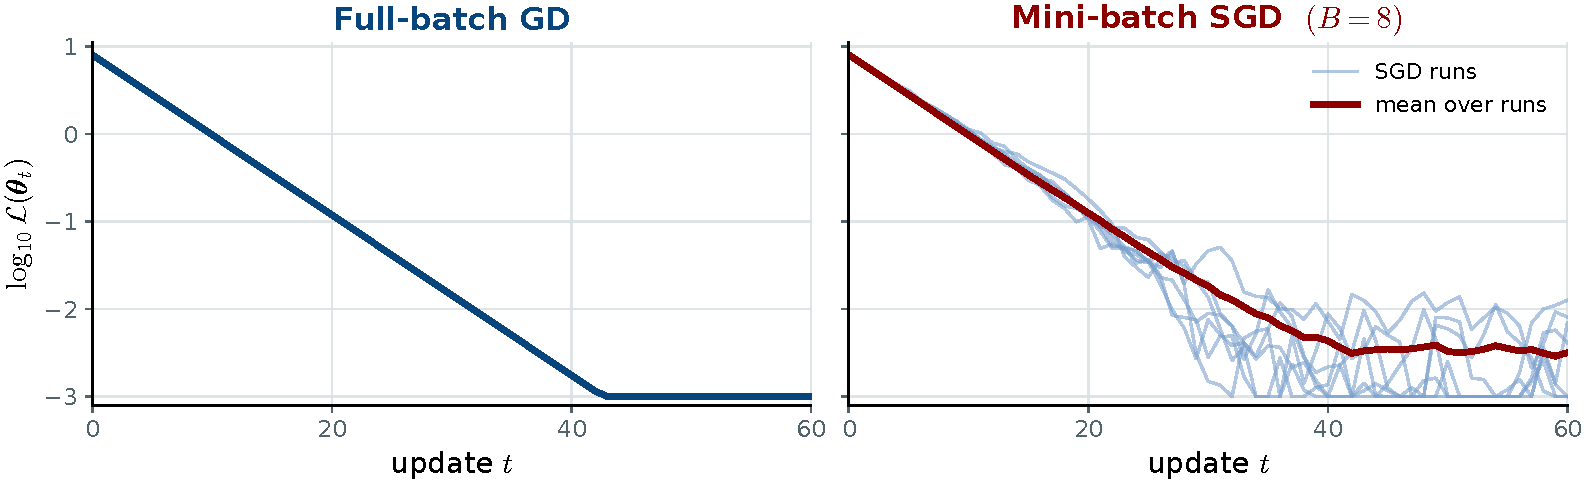
\includegraphics[width=0.92\columnwidth]{images/lecture_2/full_vs_minibatch.pdf}
		\caption{Comparison of standard GD (``full-batch'') and SGD:
			mini-batch sampling introduces noise in each update, but the loss
			still decreases on average.}
	\end{figure}

\end{whiteframe}

\begin{frame}{Extracting batches from the data}

	Instead of randomly sampling batches from the training dataset at each iteration, we generally apply the following procedure:

	\begin{enumerate}
		\item Shuffle the full dataset;
		\item Split the dataset into blocks of $B$ elements and process them sequentially, batch-by-batch;
		\item After the last block, return to point (1) and iterate.
	\end{enumerate}

	A full pass over the dataset is called an \myalert{epoch}. This is efficient because the majority of the time we deal with data stored \textit{contiguously} in memory. In practice, even the shuffling operation can be approximated.

\end{frame}

\begin{whiteframe}{Extracting batches from the data}

	\begin{figure}
		\centering
		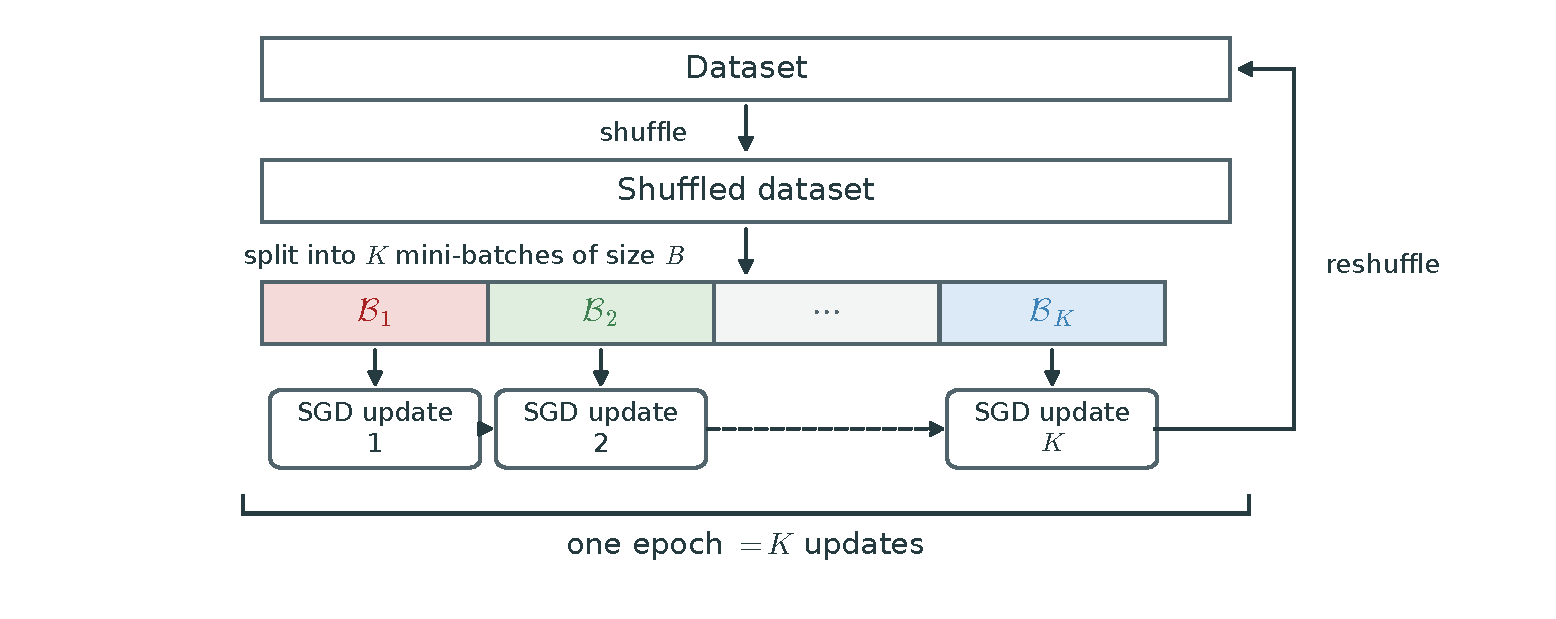
\includegraphics[width=0.82\columnwidth]{images/lecture_2/epoch_batches.pdf}
		\caption{Dividing the optimization process into epochs is also helpful to define metrics and stopping criteria.}
	\end{figure}

\end{whiteframe}

\begin{whiteframe}{Parallelizing GD optimization}

	\begin{figure}
		\centering
		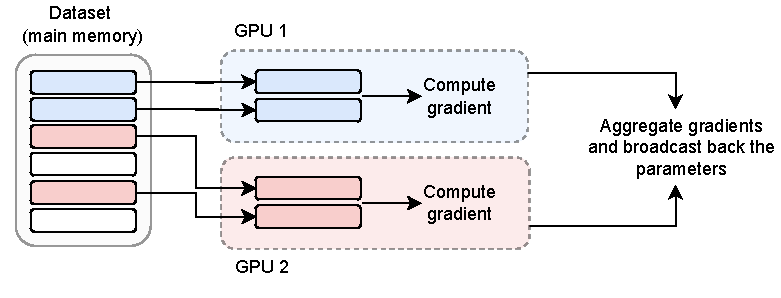
\includegraphics[width=0.7\columnwidth]{images/lecture_2/mini_batch.pdf}
		\caption{A simple form of distributed stochastic optimization: we process one mini-batch per available machine or GPU (by replicating the weights on each of them) and sum or average
			the corresponding gradients before broadcasting back the result (which is valid due to the linearity of the gradient operation). This requires a synchronization mechanism across the machines or the GPUs.}
	\end{figure}

\end{whiteframe}

\subsection{Accelerating gradient descent (optional)}

\begin{frame}{Momentum}

	Steepest-descent directions are local. On poorly conditioned objectives they can zig-zag, and noisy gradients make the path more erratic. \myalert{Momentum} smooths the path by retaining part of the previous displacement:
	%
	\vspace{-0.4cm}
	\begin{align*}
		\vc{u}_t      & =
		\underbrace{
			{\color{darkred}-\eta_t\nabla
			\widetilde{\mathcal{L}}_t(\vc{\theta}_{t-1})}
		}_{\text{\scriptsize new gradient}}
		+
		\underbrace{
			{\color{darkpastelblue}\lambda\vc{u}_{t-1}}
		}_{\text{\scriptsize retained displacement}}\,, \\
		\vc{\theta}_t & = \vc{\theta}_{t-1}+\vc{u}_t\,,
		\qquad \vc{u}_0=\vc{0},\quad 0\leq\lambda<1\,.
	\end{align*}

	\vspace{-0.54cm}

	\small Past contributions are exponentially damped: a displacement from
	$n$ iterations ago is weighted by $\lambda^{n-1}$.
	\par
	\vspace{0.05cm}

	{\centering
		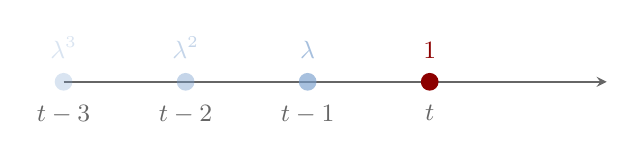
\begin{tikzpicture}[
			x=1.55cm,
			y=1cm,
			>=stealth,
			every node/.style={font=\small}
		]
			\draw[->, drawgray, line width=0.6pt]
				(0,0) -- (4.45,0);

			\foreach \x/\power/\time/\opacity in {
				0/{\lambda^3}/{t-3}/0.28,
				1/{\lambda^2}/{t-2}/0.43,
				2/{\lambda}/{t-1}/0.65
			}{
				\fill[darkpastelblue, opacity=\opacity]
					(\x,0) circle (3.2pt);
				\node[above=5pt, text=darkpastelblue, opacity=\opacity]
					at (\x,0) {$\power$};
				\node[below=5pt, text=drawgray]
					at (\x,0) {$\time$};
			}

			\fill[darkred] (3,0) circle (3.2pt);
			\node[above=5pt, text=darkred] at (3,0) {$1$};
			\node[below=5pt, text=drawgray] at (3,0) {$t$};
		\end{tikzpicture}
		\par}

\end{frame}

\begin{frame}{Adam}

	\small
	Let $\vc{g}_t=\nabla\widetilde{\mathcal{L}}_t(\vc{\theta}_{t-1})$.
	\myalert{Adam} maintains two exponential averages:

	\vspace{0.15cm}

	\begin{columns}[T,onlytextwidth]
		\begin{column}{0.48\textwidth}
			\begin{tcolorbox}[
				colback=drawblue_l!35,
				colframe=drawblue,
				boxrule=0.65pt,
				arc=1.5pt,
				left=4pt,
				right=4pt,
				top=3pt,
				bottom=4pt
			]
				\centering
				\textcolor{drawblue}{\textbf{first moment} (direction)}
				\\[0.2em]
				$\displaystyle
				\vc{m}_t=
				\beta_1\vc{m}_{t-1}+(1-\beta_1)\vc{g}_t$
			\end{tcolorbox}
		\end{column}

		\begin{column}{0.48\textwidth}
			\begin{tcolorbox}[
				colback=draworange_l!35,
				colframe=draworange,
				boxrule=0.65pt,
				arc=1.5pt,
				left=4pt,
				right=4pt,
				top=3pt,
				bottom=4pt
			]
				\centering
				\textcolor{draworange}{\textbf{second moment} (coordinate scale)}
				\\[0.2em]
				$\displaystyle
				\vc{v}_t=
				\beta_2\vc{v}_{t-1}
				+(1-\beta_2)(\vc{g}_t\odot\vc{g}_t)$
			\end{tcolorbox}
		\end{column}
	\end{columns}

	\vspace{0.08cm}

	\begin{center}
	\begin{tcolorbox}[
		width=0.72\textwidth,
		colback=drawgray_l,
		colframe=drawgray,
		boxrule=0.5pt,
		arc=1.5pt,
		left=4pt,
		right=4pt,
		top=2pt,
		bottom=4pt
	]
		\centering
		{\scriptsize\color{drawgray} bias correction (initialization at 0)}
		\\[0.15em]
		$\displaystyle
		\widehat{\vc{m}}_t=\frac{\vc{m}_t}{1-\beta_1^t}
		\qquad\qquad
		\widehat{\vc{v}}_t=\frac{\vc{v}_t}{1-\beta_2^t}$
	\end{tcolorbox}
	\end{center}

	\vspace{-0.15cm}

	\begin{center}
	\begin{tcolorbox}[
		width=0.62\textwidth,
		colback=darkred!3,
		colframe=darkred,
		boxrule=0.75pt,
		arc=1.5pt,
		left=4pt,
		right=4pt,
		top=4pt,
		bottom=4pt
	]
		\centering
		$\displaystyle
		\vc{\theta}_t=
		\vc{\theta}_{t-1}
		-\eta_t
		\frac{\widehat{\vc{m}}_t}
		{\sqrt{\widehat{\vc{v}}_t}+\varepsilon}$
	\end{tcolorbox}
	\end{center}

	\vspace{-0.35cm}

	\footnotesize
	We need to introduce two additional hyper-parameters ($\beta_1,\beta_2\in[0,1)$), but the algorithm is generally robust to their defaults (see \textbf{Muon} for more recent research).
\end{frame}

\subsection{Convexity and convergence}

\begin{frame}{Definition of a convex function}

	\myalert{Convexity} plays a pivotal role in optimization. If a function is convex, its optimization is easier with respect to a non-convex one.

	\begin{tcolorbox}
		$f$ is said to be convex if for any $\lambda \in [0,1]$:

		\vspace{0.1cm}
		\begin{columns}[T,onlytextwidth]
			\begin{column}{0.68\textwidth}
				\vspace{0.35cm}
				\begin{equation}
					\textcolor{darkgreen}{f\Bigl((1-\lambda)\vc{x}_1 + \lambda \vc{x}_2\Bigr)}
					\le
					\textcolor{darkred}{(1-\lambda)f(\vc{x}_1) + \lambda f(\vc{x}_2)} \,.
				\end{equation}

				\small
				The graph lies \textcolor{darkgreen}{below} the
				\textcolor{darkred}{chord} joining any two of its points.
			\end{column}
			\begin{column}{0.29\textwidth}
				\centering
				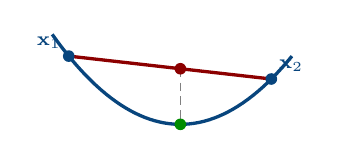
\begin{tikzpicture}[x=1.05cm,y=0.82cm]
					\draw[darkcerulean,very thick,domain=-1.55:1.35,samples=50]
						plot (\x,{0.58*(\x)^2});
					\coordinate (xone) at (-1.35,1.057);
					\coordinate (xtwo) at (1.10,0.702);
					\coordinate (chordpoint) at (0,0.861);
					\coordinate (curvepoint) at (0,0);
					\draw[darkred,very thick] (xone) -- (xtwo);
					\draw[densely dashed,gray] (chordpoint) -- (curvepoint);
					\fill[darkcerulean] (xone) circle (2.1pt)
						node[above left=-1pt] {\scriptsize $\vc{x}_1$};
					\fill[darkcerulean] (xtwo) circle (2.1pt)
						node[above right=-1pt] {\scriptsize $\vc{x}_2$};
					\fill[darkred] (chordpoint) circle (2.1pt);
					\fill[darkgreen] (curvepoint) circle (2.1pt);
				\end{tikzpicture}
			\end{column}
		\end{columns}
	\end{tcolorbox}

	If the inequality is strict for $\vc{x}_1\neq\vc{x}_2$ and $\lambda\in(0,1)$, then $f$ is \myalert{strictly convex}.

\end{frame}

\begin{frame}{Notable results on gradient descent}

	\small

	\begin{tcolorbox}[colback=light-gray,colframe=gray,
		top=1.2mm,bottom=1.2mm,left=3mm,right=3mm]
		\small
		Under standard regularity and step-size assumptions, suppose (S)GD
		converges to a stationary point $\vc{\theta}^*$.
	\end{tcolorbox}

	\vspace{-0.18cm}
	\begin{center}
		\small\textsc{More structure in $\mathcal{L}$}
		\qquad$\Longrightarrow$\qquad
		\textsc{Stronger conclusion}
	\end{center}
	\vspace{-0.25cm}

	\begin{tcolorbox}[colback=light-gray,colframe=gray,boxrule=0.7pt,
		top=0.8mm,bottom=0.8mm,left=3mm,right=3mm,arc=1.5mm]
		\begin{columns}[onlytextwidth]
			\begin{column}{0.38\textwidth}
				\textbf{Generic non-convex}
			\end{column}
			\begin{column}{0.58\textwidth}
				First-order methods generally guarantee only
				\textbf{stationarity}.
			\end{column}
		\end{columns}
	\end{tcolorbox}
	\vspace{0.06cm}
	\begin{tcolorbox}[colback=darkcerulean!6,colframe=darkcerulean,boxrule=0.7pt,
		top=0.8mm,bottom=0.8mm,left=3mm,right=3mm,arc=1.5mm]
		\begin{columns}[onlytextwidth]
			\begin{column}{0.38\textwidth}
				\textbf{Convex}
			\end{column}
			\begin{column}{0.58\textwidth}
				Every stationary point is a
				\textbf{\textcolor{darkcerulean}{global optimum}}.
			\end{column}
		\end{columns}
	\end{tcolorbox}
	\vspace{0.06cm}
	\begin{tcolorbox}[colback=darkgreen!6,colframe=darkgreen,boxrule=0.7pt,
		top=0.8mm,bottom=0.8mm,left=3mm,right=3mm,arc=1.5mm]
		\begin{columns}[onlytextwidth]
			\begin{column}{0.38\textwidth}
				\textbf{Strictly convex}
			\end{column}
			\begin{column}{0.58\textwidth}
				If an optimum exists, it is
				\textbf{\textcolor{darkgreen}{unique}}.
			\end{column}
		\end{columns}
	\end{tcolorbox}

	\vspace{-0.1cm}
	\footnotesize
	Without additional structure, globally optimizing a general non-convex
	objective can be \textbf{NP-hard}; practical first-order methods therefore
	usually target stationary points instead.

\end{frame}

\begin{frame}{Reading material}

	\textbf{Chapter 2} from the book, along with the suggested exercises.

\end{frame}

\end{document}
